%* 
%* ------------------------------------------------------------------
%* SplashWindows.tex - Creating splash windows
%* Created by Robert Heller on Thu Apr 19 14:45:52 2007
%* ------------------------------------------------------------------
%* Modification History: $Log$
%* Modification History: Revision 1.2  2007/11/30 13:56:50  heller
%* Modification History: Novemeber 30, 2007 lockdown.
%* Modification History:
%* Modification History: Revision 1.1  2007/05/06 12:49:39  heller
%* Modification History: Lock down  for 2.1.8 release candidate 1
%* Modification History:
%* Modification History: Revision 1.1  2002/07/28 14:03:50  heller
%* Modification History: Add it copyright notice headers
%* Modification History:
%* ------------------------------------------------------------------
%* Contents:
%* ------------------------------------------------------------------
%*  
%*     Model RR System, Version 2
%*     Copyright (C) 1994,1995,2002-2005  Robert Heller D/B/A Deepwoods Software
%* 			51 Locke Hill Road
%* 			Wendell, MA 01379-9728
%* 
%*     This program is free software; you can redistribute it and/or modify
%*     it under the terms of the GNU General Public License as published by
%*     the Free Software Foundation; either version 2 of the License, or
%*     (at your option) any later version.
%* 
%*     This program is distributed in the hope that it will be useful,
%*     but WITHOUT ANY WARRANTY; without even the implied warranty of
%*     MERCHANTABILITY or FITNESS FOR A PARTICULAR PURPOSE.  See the
%*     GNU General Public License for more details.
%* 
%*     You should have received a copy of the GNU General Public License
%*     along with this program; if not, write to the Free Software
%*     Foundation, Inc., 675 Mass Ave, Cambridge, MA 02139, USA.
%* 
%*  
%* 

\chapter{Creating Splash Windows}
\label{chapt:SplashWindows}
\typeout{$Id$}

Splash windows are windows that are displayed during program startup
and generally feature a company or program logo, some introductory text
and a progress meter and status text area describing the program startup
and initialization progress.

\section{Creating a Splash Window}
\begin{lstlisting}[caption={Snit spash widget creation},
		   label={lst:SPL:spashWidget}]
spash widgetpath [options...]
\end{lstlisting}
The splash widget is implemented as a Snit widget type and are created
with the spash procedure.  This widget takes eight options:\index{Splash Windows!options|(}
\begin{description}
\item[-troughcolor] The color to use for the progressbar's trough.
\item[-titleforeground] The foreground color for the title text area.
\item[-statusforeground] The foreground color for the status text area.
\item[-background] The overall background color.
\item[-progressbar] Whether or not to include a progress bar.
\item[-image] The image to display as the main feature of the spash
screen (typically a company logo or product image).
\item[-icon] A small image to display next to the title text.
\item[-title] Text to display above the main spash image.
\end{description}\index{Splash Windows!options|)}
The splash widget defines four public methods:\index{Splash Windows!methods|(}
\begin{description}
\item[update] This method takes two arguments, 
\lstinline=statusMessage percentDone=, which supply the text for the
status message and the percent of the startup that has completed.  If
the completion done percentage is 100, the spash screen's ``click to
destroy'' function is enabled.
\item[enableClickDestroy] This method enables the spash screen's ``click
to destroy'' function.
\item[hide] This method hides (withdraws) the splash window.
\item[show] This method shows (unwithdraws) the splash window.
\end{description}\index{Splash Windows!methods|)}

\section{Typical usage}

\begin{lstlisting}[caption={Typical usage},label={lst:SPL:typicalUsage}]
image create photo DeepwoodsBanner -format gif \
        -file [file join $CommonImageDir DeepwoodsBanner.gif]
# Deepwoods banner image.  Used in the splash screen.
# [index] DeepwoodsBanner!image

proc SplashScreen {} {
  # Build the ``Splash Screen'' -- A popup window that 
  # tells the user what we are all about.  It gives the 
  # version and brief copyright information.
  #
  # The upper part of the splash screen gives the brief 
  # information, with directions on how to get detailed 
  # information.  The lower part contains an image banner 
  # for Deepwoods Software.
  # [index] SplashScreen!procedure

  splash .mrrSplash \
	-title {Sample Code Program -- sample code for 
Programming Guide, Copyright (C) 2005 Robert Heller D/B/A 
Deepwoods Software Model Railroad Timetable Chart Program 
comes with ABSOLUTELY NO WARRANTY; for details select 
'Warranty...' under the Help menu.  This is free software, 
and you are welcome to redistribute it under certain 
conditions; select 'Copying...' under the Help menu.} \
        -image DeepwoodsBanner -background {#2ba2bf} \
        -titleforeground white -statusforeground {black}
}

proc SplashWorkMessage {message percent} {
  .mrrSplash update "$message" $percent
  update idle
}

wm withdraw .;# Withdraw the main window.
SplashScreen;# Create the splash screen.
update idle;# Flush pending idle events.

catch {SplashWorkMessage {Creating Main Window} 11}

# Create the main window...

catch {SplashWorkMessage {Create CTC Panel} 22}

# Create the CTC Panel...

catch {SplashWorkMessage {Create Configutation} 33}

# Create the Configutation...

catch {SplashWorkMessage {Done} 100}

\end{lstlisting}
\begin{figure}[hbpt]
\begin{centering}
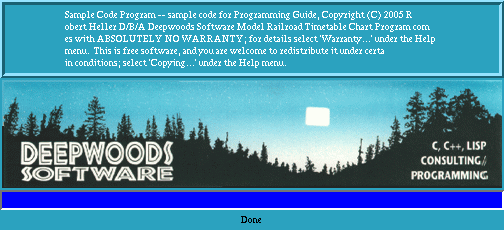
\includegraphics{SplashScreen.png}
\caption{Sample Splash Screen}
\label{fig:SPL:SplashScreen}
\end{centering}
\end{figure}
Listing~\ref{lst:SPL:typicalUsage} shows how a splash window is
typically created and updated.  The procedure in lines 6-28 creates the
splash window and the procedure in lines 29-32 updates the status text
area and progress bar.  After withdrawing the main window, the splash
window is created and drawn (lines 34-36).  As progress is made during
program startup, the splash window is updates (lines 38, 42, 46, and
50). When the percent completed is set to 100, the splash window can be
removed when the user left-clicks anywhere on it.  The splash window this
code creates is shown in Figure~\ref{fig:SPL:SplashScreen}.

